\section{Đóng gói mô hình}
\subsection{Khả năng ứng dụng thực tế}
Với mô hình nhận diện và phân loại các sản phẩm về thời trang này, nếu được phát triển tốt hơn nữa thì nó có thể được đưa vào hệ thống của các trang thương mại điện tử như Shopee, Lazada, ...Ví dụ như khi các nhà bán hàng đăng tải thông tin và hình ảnh của 1 sản phẩm nào đó lên các sàn thương mại, khi đó thay vì phải tự lựa chọn xem chúng thuộc vào loại danh mục nào thì chúng ta chỉ cần tải lên và hệ thống sẽ tự động cập nhật vào danh sách các sản phẩm phù hợp.\\

Ngoài ra, dựa vào kết quả dự đoán của mô hình này thì ta cũng có thể tạo ra một hệ thống gợi ý các sản phẩm tương tự, ví dụ như hình dưới đây:
\begin{center}
    \begin{figure}[!h]
        \centering
        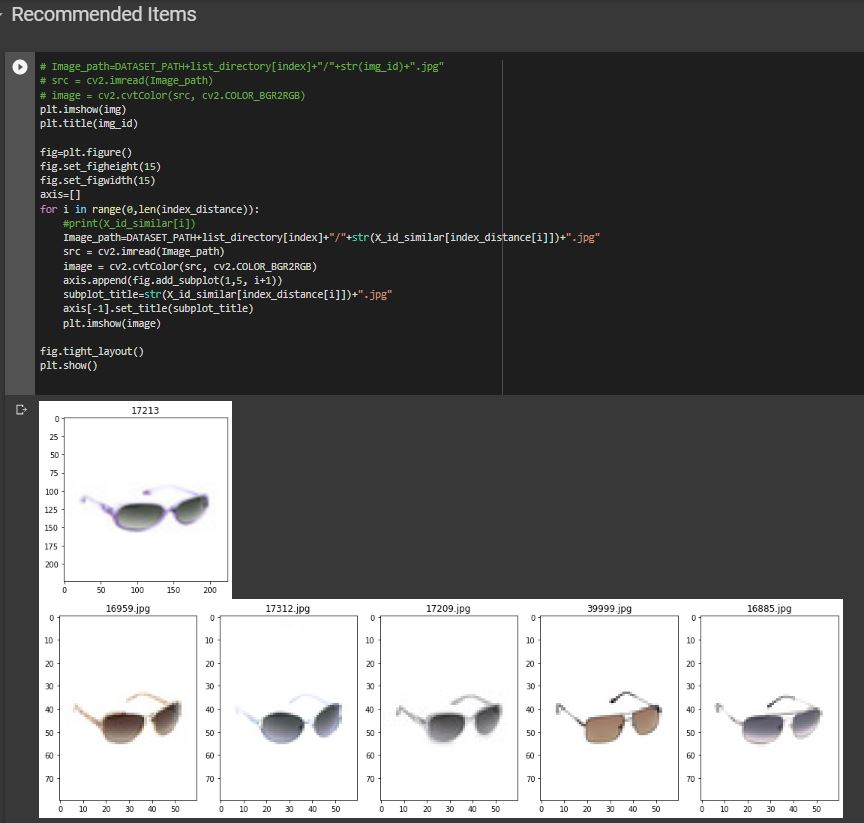
\includegraphics[scale = 0.8]{fileanh/41.jpg}
        \caption{Recommended items}
    \end{figure}
\end{center}


\subsection{Mô hình tiên tiến}
Sử dụng mô hình \textbf{EfficientNetV2L} được trình bày trong paper \href{https://arxiv.org/abs/2104.00298}{\textit{EfficientNetV2: Smaller Models and Faster Training (ICML 2021)}}